%!TEX program = xelatex
% ==============================================================================
% AA CONFIGURAZIONE DI BASE ED ENGINE
% ==============================================================================
% BB CLASSE DEL DOCUMENTO
\documentclass[11pt, a4paper]{article}

% ==============================================================================
% AA LINGUA, FONT E TIPOGRAFIA
% ==============================================================================
% BB GESTIONE FONT XELATEX
\usepackage{fontspec}
\setmainfont{Latin Modern Roman}

% BB LOCALIZZAZIONE LINGUISTICA
\usepackage[italian]{babel}

% BB TIPOGRAFIA E MICRO-ESTENSIONI
\usepackage[protrusion=true]{microtype}
\raggedbottom

% ==============================================================================
% AA LAYOUT DI PAGINA E SPAZIATURA PARAGRAFI
% ==============================================================================
% BB GEOMETRIA DEI MARGINI
\usepackage[left=2.4cm, right=1.6cm, top=2cm, bottom=2cm]{geometry}

% BB CONTROLLO SPAZIATURA TRA PARAGRAFI
\usepackage[skip=3pt plus 1pt minus 1pt]{parskip}

% ==============================================================================
% AA MOTORE DEI COLORI E MACRO LOCALI
% ==============================================================================
% BB CARICAMENTO CORE XCOLOR IN SPAZIO GRAY PURO
\usepackage[gray]{xcolor}

% ==============================================================================
% AA MATEMATICA E SIMBOLI SCIENTIFICI
% ==============================================================================
% BB PACCHETTI MATEMATICI UNICODE
\usepackage{mathtools}
\usepackage[warnings-off={mathtools-overbracket,mathtools-colon}]{unicode-math}
\setmathfont{Latin Modern Math}

% BB METRICHE MATRICI E FORMULE DISPLAY
\setlength{\arraycolsep}{10pt}
\setlength{\abovedisplayskip}{3pt plus 1pt minus 1pt}
\setlength{\belowdisplayskip}{3pt plus 1pt minus 1pt}
\setlength{\abovedisplayshortskip}{0pt plus 1pt}
\setlength{\belowdisplayshortskip}{2pt plus 1pt minus 1pt}
\allowdisplaybreaks

% ==============================================================================
% AA GRAFICA ED ELEMENTI FLOTTANTI
% ==============================================================================
% BB MOTORE DI INCLUSIONE GRAFICA E GESTIONE RIGIDA
\usepackage{graphicx}
\graphicspath{{./E4_6_2_Images/}}
\usepackage{float}

% ==============================================================================
% AA TITOLI E STRUTTURA DEL DOCUMENTO (MONOCROMATICI NERI)
% ==============================================================================
% BB PACCHETTO TITLESEC
\usepackage{titlesec}

% BB FORMATTAZIONE TIPOGRAFICA (TITOLI NERI)
\titleformat{\section}{\normalfont\Large\bfseries}{\thesection}{1em}{}
\titleformat{name=\section,numberless}{\normalfont\Large\bfseries}{}{0pt}{}
\titleformat{\subsection}{\normalfont\large\bfseries}{\thesubsection}{1em}{}
\titleformat{name=\subsection,numberless}{\normalfont\large\bfseries}{}{0pt}{}
\titleformat{\subsubsection}{\normalfont\normalsize\bfseries}{\thesubsubsection}{1em}{}
\titleformat{name=\subsubsection,numberless}{\normalfont\normalsize\bfseries}{}{0pt}{}

% BB SPAZIATURA VERTICALE DEI TITOLI
\titlespacing*{\section}{0pt}{1.2ex plus 0.4ex minus 0.2ex}{0.6ex plus 0.2ex}
\titlespacing*{\subsection}{0pt}{1ex plus 0.3ex minus 0.2ex}{0.5ex plus 0.2ex}
\titlespacing*{\subsubsection}{0pt}{0.8ex plus 0.2ex minus 0.1ex}{0.4ex plus 0.1ex}

% ==============================================================================
% AA INTEGRAZIONE AMBIENTE MATLAB
% ==============================================================================
% BB CARICAMENTO PACCHETTO MATLAB
\usepackage{matlab}

% BB ATTIVAZIONE SEGNALIBRI E INDICE MATLAB
\matlabmultipletitles
\matlabhastoc

% ==============================================================================
% AA IPERTESTO, SEGNALIBRI ED ELENCHI
% ==============================================================================
% BB CONFIGURAZIONE HYPERREF E METADATI PDF
\hypersetup{
    hidelinks,
    pdfauthor={Francesco Lo Verde},
    pdftitle={Disaccoppiamento polso struttura portante}
}

% BB SEGNALIBRI AVANZATI
\usepackage{bookmark}

% BB FORMATTAZIONE ELENCHI PUNTATI E NUMERATI
\usepackage{enumitem}
\setlist{itemsep=3.5pt plus 1pt minus 1pt, topsep=4pt plus 1pt minus 1pt, partopsep=0pt, parsep=1pt}

\begin{document}
\matlabtitle{\texorpdfstring{Disaccoppiamento polso-struttura portante nel manipolatore di\\ Stanford}{Disaccoppiamento polso-struttura portante manipolatore di Stanford}}
\subsection*{Cinematica diretta della struttura portante sferica}

\begin{par}
    \begin{figure}[!htbp]
        \centering
        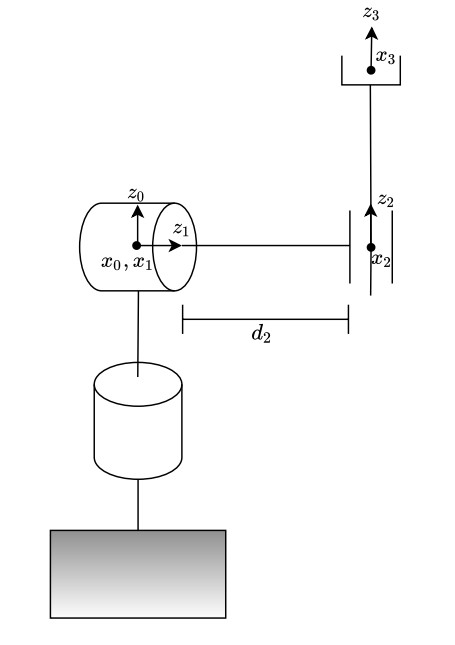
\includegraphics[width=0.25\linewidth]{image_0.jpeg}
    \end{figure}
\end{par}

\begin{matlabcode}
clc; clear; close all;

% Definizione variabili simboliche
syms q1 q2 q3 d2 real;
DH_table_Strut = [q1, 0, -pi/2, 0;
                  q2, d2, pi/2, 0;
                  0, q3, 0, 0];

% Numero giunti manipolatore
n = size(DH_table_Strut, 1);
% Calcolo matrici trasformazione struttura
[A_matrices_Strut, R_matrices_Strut] = Compute_DH_Transformations(DH_table_Strut);
% Visualizzazione matrici trasformazione struttura
j = 0;
for i = 1:n
    fprintf('Matrice di trasformazione omogenea ^(%d)A_(%d):\n', j, j+1);
    disp(A_matrices_Strut(:,:,i));
    j = j+1;
end
\end{matlabcode}
\begin{matlaboutput}
Matrice di trasformazione omogenea ^(0)A_(1):
\end{matlaboutput}
\begin{matlabsymbolicoutput}
$\displaystyle \left(\begin{array}{cccc}
\cos \left(q_1 \right) & 0 & -\sin \left(q_1 \right) & 0\\
\sin \left(q_1 \right) & 0 & \cos \left(q_1 \right) & 0\\
0 & -1 & 0 & 0\\
0 & 0 & 0 & 1
\end{array}\right)$
\end{matlabsymbolicoutput}

\begin{matlaboutput}
Matrice di trasformazione omogenea ^(1)A_(2):
\end{matlaboutput}
\begin{matlabsymbolicoutput}
$\displaystyle \left(\begin{array}{cccc}
\cos \left(q_2 \right) & 0 & \sin \left(q_2 \right) & 0\\
\sin \left(q_2 \right) & 0 & -\cos \left(q_2 \right) & 0\\
0 & 1 & 0 & d_2 \\
0 & 0 & 0 & 1
\end{array}\right)$
\end{matlabsymbolicoutput}
\begin{matlaboutput}
Matrice di trasformazione omogenea ^(2)A_(3):
\end{matlaboutput}
\begin{matlabsymbolicoutput}
$\displaystyle \left(\begin{array}{cccc}
1 & 0 & 0 & 0\\
0 & 1 & 0 & 0\\
0 & 0 & 1 & q_3 \\
0 & 0 & 0 & 1
\end{array}\right)$
\end{matlabsymbolicoutput}
\newpage
\begin{matlabcode}
% Calcolo matrice di trasformazione omogenea da base a centro del polso
T03 = A_matrices_Strut(:,:,1) * A_matrices_Strut(:,:,2) * A_matrices_Strut(:,:,3);
T03 = simplify(T03);

fprintf('Matrice di trasformazione omogenea ^(0)T_(3):\n');

disp(T03);
\end{matlabcode}
\begin{matlaboutput}
Matrice di trasformazione omogenea ^(0)T_(3):
\end{matlaboutput}
\[
    ^{0}\mathbf{T}_{3}(\mathbf{q}) \; = \; ^{0}\mathbf{A}_{1}(q_{1}) \; \cdot \; ^{1}\mathbf{A}_{2}(q_{2}) \; \cdot \; ^{2}\mathbf{A}_{3}(q_{3}) =
\]

\[
    =
    \begin{pmatrix}
        c(q_{1})c(q_{2}) & -s(q_{1}) & c(q_{1})s(q_{2}) & c(q_{1})s(q_{2})q_{3} - s(q_{1})d_{2} \\
        s(q_{1})c(q_{2}) & c(q_{1}) & s(q_{1})s(q_{2}) & s(q_{1})s(q_{2})q_{3} + c(q_{1})d_{2}\\
        -s(q_{2}) & 0 & c(q_{2}) & c(q_{2})q_{3}\\
        0 & 0 & 0 & 1
    \end{pmatrix}
\]
\subsection*{Cinematica diretta del polso sferico}
\begin{par}
    \begin{figure}[htbp]
        \centering
        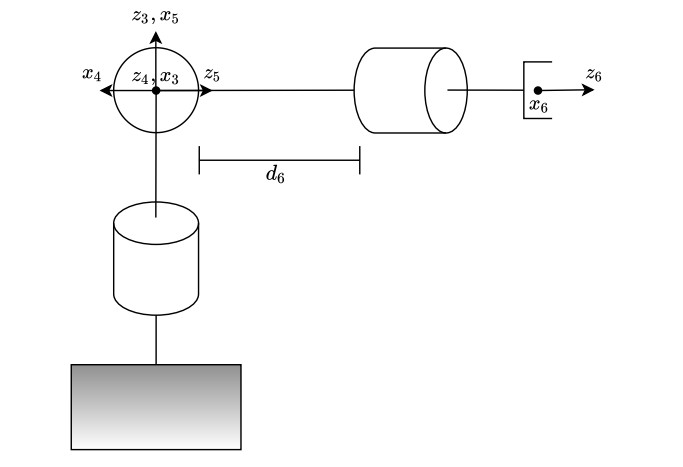
\includegraphics[width=0.375\linewidth]{image_1.jpeg}
    \end{figure}
\end{par}

\begin{matlabcode}
% Definizione variabili simboliche
syms q4 q5 q6 d6 real;
% Tabella parametri Denavit-Hartenberg (DH)
DH_table_Polso = [q4, 0, -pi/2, 0;
                  q5, 0, pi/2, 0;
                  q6, d6, 0, 0];

% Numero giunti manipolatore
n = size(DH_table_Polso, 1);
% Calcolo matrici trasformazione polso
[A_matrices_Polso, R_matrices_Polso] = Compute_DH_Transformations(DH_table_Polso);

% Visualizzazione matrici trasformazione polso
j = 3;
for i = 1:n
    fprintf('Matrice di trasformazione omogenea ^(%d)A_(%d):\n', j, j+1);
    disp(A_matrices_Polso(:,:,i));

    j = j+1;
end
\end{matlabcode}
\newpage
\begin{matlaboutput}
Matrice di trasformazione omogenea ^(3)A_(4):
\end{matlaboutput}
\begin{matlabsymbolicoutput}
$\displaystyle \left(\begin{array}{cccc}
\cos \left(q_4 \right) & 0 & -\sin \left(q_4 \right) & 0\\
\sin \left(q_4 \right) & 0 & \cos \left(q_4 \right) & 0\\
0 & -1 & 0 & 0\\
0 & 0 & 0 & 1
\end{array}\right)$
\end{matlabsymbolicoutput}
\begin{matlaboutput}
Matrice di trasformazione omogenea ^(4)A_(5):
\end{matlaboutput}
\begin{matlabsymbolicoutput}
$\displaystyle \left(\begin{array}{cccc}
\cos \left(q_5 \right) & 0 & \sin \left(q_5 \right) & 0\\
\sin \left(q_5 \right) & 0 & -\cos \left(q_5 \right) & 0\\
0 & 1 & 0 & 0\\
0 & 0 & 0 & 1
\end{array}\right)$
\end{matlabsymbolicoutput}
\begin{matlaboutput}
Matrice di trasformazione omogenea ^(5)A_(6):
\end{matlaboutput}
\begin{matlabsymbolicoutput}
$\displaystyle \left(\begin{array}{cccc}
\cos \left(q_6 \right) & -\sin \left(q_6 \right) & 0 & 0\\
\sin \left(q_6 \right) & \cos \left(q_6 \right) & 0 & 0\\
0 & 0 & 1 & d_6 \\
0 & 0 & 0 & 1
\end{array}\right)$
\end{matlabsymbolicoutput}

\begin{matlabcode}
% Calcolo matrice di trasformazione omogenea da centro del polso a end-effector
T36 = A_matrices_Polso(:,:,1) * A_matrices_Polso(:,:,2) * A_matrices_Polso(:,:,3);
T36 = simplify(T36);

fprintf('Matrice di trasformazione omogenea ^(3)T_(6):\n');

disp(T36);
\end{matlabcode}
\begin{matlaboutput}
Matrice di trasformazione omogenea ^(3)T_(6):
\end{matlaboutput}
\[
    ^{3}\mathbf{T}_{6}(\mathbf{q}) \; = \; ^{3}\mathbf{A}_{4}(q_{4}) \; \cdot \; ^{4}\mathbf{A}_{5}(q_{5}) \; \cdot \; ^{5}\mathbf{A}_{6}(q_{6}) =
\]
\[
    =
        \begin{pmatrix}
            c(q_{4})c(q_{5})c(q_{6}) - s(q_{4})s(q_{6}) & -c(q_{6})s(q_{4}) - c(q_{4})c(q_{5})s(q_{6}) & c(q_{4})s(q_{5}) & c(q_{4})s(q_{5})d_{6} \\
            c(q_{4})s(q_{6}) + c(q_{5})c(q_{6})s(q_{4}) & c(q_{4})c(q_{6}) - c(q_{5})s(q_{4})s(q_{6}) & s(q_{4})s(q_{5}) & s(q_{4})s(q_{5})d_{6} \\
            -c(q_{6})s(q_{5}) & s(q_{5})s(q_{6}) & c(q_{5}) & c(q_{5})d_{6} \\
            0 & 0 & 0 & 1
        \end{pmatrix}
\]

\subsection*{Cinematica diretta completa del manipolatore di Stanford}
\begin{matlabcode}
% Calcolo matrice di trasformazione totale da base a end-effector
T06 = T03 * T36;
\end{matlabcode}

\begin{par}
\begin{flushleft}
Vedere Appendice E3.6.2.A -- Matrice di trasformazione omogenea completa ${}^{0}T_{6}$.
\end{flushleft}
\end{par}

\subsection*{Verifica della condizione di disaccoppiamento cinematico}

\begin{par}
$$\exists \;{\mathbf{d}}_0 ,\,{\mathbf{d}}_1 \in {\mathbb{R}}^3 \;\;\mid \;\;^3 {\mathbf{d}}_6 =^3 {\mathbf{R}}_6 {\mathbf{d}}_1 +{\mathbf{d}}_0$$
\end{par}

\begin{matlabcode}
% Estrazione vettore posizione
d36 = T36(1:3, 4);
d36 = simplify(d36);
fprintf('Vettore posizione ^(3)d_(6):\n');

disp(d36);
\end{matlabcode}
\begin{matlaboutput}
Vettore posizione ^(3)d_(6):
\end{matlaboutput}

\begin{matlabsymbolicoutput}
$\displaystyle \left(\begin{array}{c}
d_6 \,\cos \left(q_4 \right)\,\sin \left(q_5 \right)\\
d_6 \,\sin \left(q_4 \right)\,\sin \left(q_5 \right)\\
d_6 \,\cos \left(q_5 \right)
\end{array}\right)$
\end{matlabsymbolicoutput}
\newpage
\begin{matlabcode}
% Verifica vettori costanti d_0 e d_1 (Condizione di Pieper)
d0 = [0; 0; 0];
R36_polso = simplify(T36(1:3, 1:3));
d1 = simplify(transpose(R36_polso) * d36);
fprintf('Vettore d_(0):\n');
disp(d0);
fprintf('Vettore d_(1) = (^(3)R_(6))^(T) ^(3)d_(6):\n');
disp(d1);
\end{matlabcode}
\begin{matlaboutput}
Vettore d_(0):
     0
     0
     0
Vettore d_(1) = (^(3)R_(6))^(T) ^(3)d_(6):
\end{matlaboutput}
\begin{matlabsymbolicoutput}
$\displaystyle
    \begin{pmatrix}
        0\\
        0\\
        d_{6}
    \end{pmatrix}
$
\end{matlabsymbolicoutput}

\subsection*{Cinematica inversa di posizione della struttura portante}

\begin{par}
$$^0 {\mathbf{d}}_6 =^0 {\mathbf{d}}_3 +^0 {\mathbf{R}}_3 {\,}^3 {\mathbf{d}}_6$$
\end{par}

\begin{matlabcode}
% Estrazione vettore posizione
d03 = T03(1:3, 4);
d03 = simplify(d03);
fprintf('Vettore posizione ^(0)d_(3):\n');

disp(d03);
\end{matlabcode}
\begin{matlaboutput}
Vettore posizione ^(0)d_(3):
\end{matlaboutput}
\begin{matlabsymbolicoutput}
$\displaystyle \left(\begin{array}{c}
q_3 \,\cos \left(q_1 \right)\,\sin \left(q_2 \right)-d_2 \,\sin \left(q_1 \right)\\
d_2 \,\cos \left(q_1 \right)+q_3 \,\sin \left(q_1 \right)\,\sin \left(q_2 \right)\\
q_3 \,\cos \left(q_2 \right)
\end{array}\right)$
\end{matlabsymbolicoutput}

\begin{matlabcode}
% Isolamento posizione desiderata del centro polso e risoluzione (q3, q2, q1)
syms dx dy dz d03HatNormSq real;
d06_des = [dx; dy; dz];
R06_des = sym('r06_', [3, 3], 'real');
d03_hat = simplify(d06_des - R06_des * d1);
fprintf('Vettore desiderato centro del polso d03_hat = ^(0)d_(6) - ^(0)R_(6) d_(1):\n');
disp(d03_hat);
\end{matlabcode}
\begin{matlaboutput}
Vettore desiderato centro del polso d03_hat = ^(0)d_(6) - ^(0)R_(6) d_(1):
\end{matlaboutput}
\begin{matlabsymbolicoutput}
$\displaystyle \left(\begin{array}{c}
\textrm{dx}-d_6 \,r_{06,1,3} \\
\textrm{dy}-d_6 \,r_{06,2,3} \\
\textrm{dz}-d_6 \,r_{06,3,3}
\end{array}\right)$
\end{matlabsymbolicoutput}
\begin{matlabcode}
q3_sol_pos = sqrt(d03HatNormSq - d2^2);
q3_sol_neg = -sqrt(d03HatNormSq - d2^2);
cos_q2 = d03_hat(3) / q3;
q2_sol_pos = atan2(sqrt(1 - cos_q2^2), cos_q2);
q2_sol_neg = atan2(-sqrt(1 - cos_q2^2), cos_q2);

A_q1 = [q3*sin(q2), -d2; d2, q3*sin(q2)];
cs_q1 = simplify(inv(A_q1) * [d03_hat(1); d03_hat(2)]);
q1_sol = atan2(cs_q1(2), cs_q1(1));
\end{matlabcode}
\newpage
\begin{matlabcode}
fprintf('Soluzioni simboliche (q3, q2, q1):\n');
fprintf('q3 (+):\n'); disp(q3_sol_pos);
fprintf('q3 (-):\n'); disp(q3_sol_neg);
fprintf('q2 (+):\n'); disp(q2_sol_pos);
fprintf('q2 (-):\n'); disp(q2_sol_neg);
fprintf('q1:\n'); disp(q1_sol);
\end{matlabcode}
\begin{matlaboutput}
Soluzioni simboliche (q3, q2, q1):
q3 (+):
\end{matlaboutput}
\begin{matlabsymbolicoutput}
$\displaystyle \sqrt{\textrm{d03HatNormSq}-{d_2}^2}$
\end{matlabsymbolicoutput}
\begin{matlaboutput}
q3 (-):
\end{matlaboutput}
\begin{matlabsymbolicoutput}
$\displaystyle -\sqrt{\textrm{d03HatNormSq}-{d_2}^2}$
\end{matlabsymbolicoutput}
\begin{matlaboutput}
q2 (+):
\end{matlaboutput}
\begin{matlabsymbolicoutput}
\resizebox{\ifdim\width>\linewidth\linewidth\else\width\fi}{!}{%
$\displaystyle \textrm{atan2}\left(\sqrt{1-\frac{{\left(\textrm{dz}-d_6\,r_{06,3,3}\right)}^2}{{q_3}^2}}, \frac{\textrm{dz}-d_6\,r_{06,3,3}}{q_3}\right)$}
\end{matlabsymbolicoutput}
\begin{matlaboutput}
q2 (-):
\end{matlaboutput}
\begin{matlabsymbolicoutput}
\resizebox{\ifdim\width>\linewidth\linewidth\else\width\fi}{!}{%
$\displaystyle \textrm{atan2}\left(-\sqrt{1-\frac{{\left(\textrm{dz}-d_6\,r_{06,3,3}\right)}^2}{{q_3}^2}}, \frac{\textrm{dz}-d_6\,r_{06,3,3}}{q_3}\right)$}
\end{matlabsymbolicoutput}
\begin{matlaboutput}
q1:
\end{matlaboutput}
\begin{matlabsymbolicoutput}
\resizebox{\ifdim\width>\linewidth\linewidth\else\width\fi}{!}{%
$\displaystyle \textrm{atan2}\left(\frac{q_3\,\sin(q_2)\,(\textrm{dy}-d_6\,r_{06,2,3})-d_2\,(\textrm{dx}-d_6\,r_{06,1,3})}{{d_2}^2+{q_3}^2\,\sin(q_2)^2}, \frac{d_2\,(\textrm{dy}-d_6\,r_{06,2,3})+q_3\,\sin(q_2)\,(\textrm{dx}-d_6\,r_{06,1,3})}{{d_2}^2+{q_3}^2\,\sin(q_2)^2}\right)$}
\end{matlabsymbolicoutput}

\subsection*{Cinematica inversa di orientamento del polso sferico}

\[
    {}^{0}\mathbf{R}_6 = {}^{0}\mathbf{R}_3 \cdot {}^{3}\mathbf{R}_{6}
\]

\begin{matlabcode}
% Matrice di rotazione R06
T06 = simplify(T03 * T36);
R06 = T06(1:3, 1:3);
R06 = simplify(R06);
% Matrice di rotazione R03 trasposta
R03 = T03(1:3, 1:3);
R03 = simplify(R03);
R03_T = transpose(R03);
% Matrice di rotazione R36 calcolata
R36 = R03_T * R06;
R36 = simplify(R36);
fprintf('Matrice di rotazione R36 = (R03)^(T) R06 =\n');
disp(R36);
\end{matlabcode}
\begin{matlaboutput}
Matrice di rotazione R36 = (R03)^(T) R06 =
\end{matlaboutput}
\begin{matlabsymbolicoutput}
\resizebox{0.9\linewidth}{!}{%
$\displaystyle \begin{pmatrix}
    \cos \left(q_4 \right)\,\cos \left(q_5 \right)\,\cos \left(q_6 \right)-\sin \left(q_4 \right)\,\sin \left(q_6 \right) & -\cos \left(q_6 \right)\,\sin \left(q_4 \right)-\cos \left(q_4 \right)\,\cos \left(q_5 \right)\,\sin \left(q_6 \right) & \cos \left(q_4 \right)\,\sin \left(q_5 \right)\\
    \cos \left(q_4 \right)\,\sin \left(q_6 \right)+\cos \left(q_5 \right)\,\cos \left(q_6 \right)\,\sin \left(q_4 \right) & \cos \left(q_4 \right)\,\cos \left(q_6 \right)-\cos \left(q_5 \right)\,\sin \left(q_4 \right)\,\sin \left(q_6 \right) & \sin \left(q_4 \right)\,\sin \left(q_5 \right)\\
    -\cos \left(q_6 \right)\,\sin \left(q_5 \right) & \sin \left(q_5 \right)\,\sin \left(q_6 \right) & \cos \left(q_5 \right)
\end{pmatrix}$%
}
\end{matlabsymbolicoutput}

\begin{matlabcode}
% Matrice nota R_bar = (^(0)R_(3))^(T) R06_hat e soluzioni (q5, q4, q6)
R03_K = sym('r03_', [3, 3], 'real');
R_bar_calc = transpose(R03_K) * R06_des;
R_bar = sym('r_bar', [3, 3], 'real');
cos_q5 = R_bar(3,3);
q5_sol_pos = atan2(sqrt(1 - cos_q5^2), cos_q5);
q5_sol_neg = atan2(-sqrt(1 - cos_q5^2), cos_q5);
q4_sol = atan2(R_bar(2,3) / sin(q5), R_bar(1,3) / sin(q5));
q6_sol = atan2(R_bar(3,2) / sin(q5), -R_bar(3,1) / sin(q5));
fprintf('Soluzioni simboliche (q5, q4, q6):\n');
fprintf('q5 (+):\n'); disp(q5_sol_pos);
fprintf('q5 (-):\n'); disp(q5_sol_neg);
fprintf('q4:\n'); disp(q4_sol);
fprintf('q6:\n'); disp(q6_sol);
\end{matlabcode}
\begin{matlaboutput}
Soluzioni simboliche (q5, q4, q6):
q5 (+):
\end{matlaboutput}
\begin{matlabsymbolicoutput}
$\displaystyle \textrm{atan2}\left(\sqrt{1-{r_{\textrm{bar3},3}}^2}, r_{\textrm{bar3},3}\right)$
\end{matlabsymbolicoutput}
\begin{matlaboutput}
q5 (-):
\end{matlaboutput}
\begin{matlabsymbolicoutput}
$\displaystyle \textrm{atan2}\left(-\sqrt{1-{r_{\textrm{bar3},3}}^2}, r_{\textrm{bar3},3}\right)$
\end{matlabsymbolicoutput}
\begin{matlaboutput}
q4:
\end{matlaboutput}
\begin{matlabsymbolicoutput}
$\displaystyle \textrm{atan2}\left(\frac{r_{\textrm{bar2},3}}{\sin(q_5)}, \frac{r_{\textrm{bar1},3}}{\sin(q_5)}\right)$
\end{matlabsymbolicoutput}
\begin{matlaboutput}
q6:
\end{matlaboutput}
\begin{matlabsymbolicoutput}
$\displaystyle \textrm{atan2}\left(\frac{r_{\textrm{bar3},2}}{\sin(q_5)}, -\frac{r_{\textrm{bar3},1}}{\sin(q_5)}\right)$
\end{matlabsymbolicoutput}

\matlabheading{Analisi del caso singolare del polso \texorpdfstring{$\sin (q_5 )=0$}{sin(q5) = 0}}

\matlabheadingtwo{Configurazione singolare con \texorpdfstring{$q_5 =0$}{q5 = 0}}

\begin{matlabcode}
% Sostituzione q5 = 0
R36_Zero = subs(R36, q5, 0);
R36_Zero = simplify(R36_Zero);

fprintf('Matrice di rotazione R36 calcolata con q5 = 0:\n');

disp(R36_Zero);
\end{matlabcode}
\begin{matlaboutput}
Matrice di rotazione R36 calcolata con q5 = 0:
\end{matlaboutput}

\begin{matlabsymbolicoutput}
$\displaystyle \left(\begin{array}{ccc}
\cos \left(q_4 +q_6 \right) & -\sin \left(q_4 +q_6 \right) & 0\\
\sin \left(q_4 +q_6 \right) & \cos \left(q_4 +q_6 \right) & 0\\
0 & 0 & 1
\end{array}\right)$
\end{matlabsymbolicoutput}
\begin{matlabcode}
q4_plus_q6 = atan2(R_bar(2,1), R_bar(1,1));
fprintf('In singolarità q5 = 0, q4 + q6 =\n');
disp(q4_plus_q6);
\end{matlabcode}
\begin{matlaboutput}
In singolarità q5 = 0, q4 + q6 =
\end{matlaboutput}
\begin{matlabsymbolicoutput}
$\displaystyle \textrm{atan2}\left(r_{\textrm{bar2},1} ,r_{\textrm{bar1},1} \right)$
\end{matlabsymbolicoutput}
Dove:
\begin{align*}
    r_{\textrm{bar2},1} &= \sin(q_{4} + q_{6}) \\
    r_{\textrm{bar1},1} &= \cos(q_{4} + q_{6})
\end{align*}
\newpage
\matlabheadingtwo{Configurazione singolare con \texorpdfstring{$q_5 =\pi$}{q5 = pi}}

\begin{matlabcode}
% Sostituzione q5 = pi
R36_Pi = subs(R36, q5, pi);
R36_Pi = simplify(R36_Pi);

fprintf('Matrice di rotazione R36 calcolata con q5 = pi:\n');

disp(R36_Pi);
\end{matlabcode}
\begin{matlaboutput}
Matrice di rotazione R36 calcolata con q5 = pi:
\end{matlaboutput}
\begin{matlabsymbolicoutput}
$\displaystyle \left(\begin{array}{ccc}
-\cos \left(q_4 -q_6 \right) & -\sin \left(q_4 -q_6 \right) & 0\\
-\sin \left(q_4 -q_6 \right) & \cos \left(q_4 -q_6 \right) & 0\\
0 & 0 & -1
\end{array}\right)$
\end{matlabsymbolicoutput}
\begin{matlabcode}
q4_minus_q6 = atan2(-R_bar(2,1), R_bar(2,2));
fprintf('In singolarità q5 = pi, q4 - q6 =\n');
disp(q4_minus_q6);
\end{matlabcode}
\begin{matlaboutput}
In singolarità q5 = pi, q4 - q6 =
\end{matlaboutput}
\begin{matlabsymbolicoutput}
$\displaystyle \textrm{atan2}\left(-r_{\textrm{bar2},1} ,r_{\textrm{bar2},2} \right)$
\end{matlabsymbolicoutput}
Dove:
\begin{align*}
    -r_{\textrm{bar2},1} &= \sin(q_{4} - q_{6}) \\
    r_{\textrm{bar2},2} &= \cos(q_{4} - q_{6})
\end{align*}

\end{document}
